\documentclass{article}

\usepackage{neurips_2026}

\usepackage[utf8]{inputenc}
\usepackage[T2A,T1]{fontenc}
\usepackage[english,russian]{babel}
\usepackage{tempora} % Times-совместимый шрифт с кириллицей (T2A); ptm не содержит T2A
\renewcommand{\sfdefault}{PTSans-TLF} % sans с кириллицей вместо phv (Helvetica без T2A)
\usepackage{hyperref}
\hypersetup{unicode=true}
\usepackage{url}
\usepackage{booktabs}
\usepackage{amsfonts}
\usepackage{amssymb}
\usepackage{amsmath}
\usepackage{nicefrac}
\usepackage{microtype}
\usepackage{xcolor}
\usepackage{graphicx}
\usepackage{array}
\usepackage{enumitem}
\usepackage{placeins}

\newcommand{\method}[1]{\texttt{#1}}
\newcommand{\wstar}{W^{\star}}
\newcommand{\rwstar}{RW^{\star}}
\newcommand{\mstar}{M^{\star}}
\newcommand{\cstar}{C^{\star}}
\newcommand{\phiroute}{\varphi_{\mathrm{route}}}

% TODO(camera-ready): venue retarget; cite the three companion papers
% (Q/R/M/C framework, collective semantic memory, semantic warp) per the
% venue's concurrent-submission policy.

\title{Песня, а не точка: перенос маршрутов и\\смысловая идентичность мест в коллективной памяти}

%\author{%
%  Anonymous Authors \\
%}

\begin{document}

\maketitle

\begin{abstract}
\textbf{Проблема.} Сопутствующая статья о варпе измеряет, способен ли
агент достичь цели, известной лишь из памяти напарника. В этой
конструкции --- и, по существу, во всех мультиагентных системах с общей
памятью --- скрыты два допущения. Во-первых, переносится \emph{точка}:
широковещательные снимки несут сводки мест, но не рёбра, поэтому путник
(traveler) узнаёт ГДЕ и вынужден заново выводить КАК. Во-вторых,
идентичность места задаётся \emph{общей системой координат}: <<то же
место>> означает <<близкие $(x,y)$ в сетке, которую среда выдаёт каждому
агенту>>; семантика лишь разрешает конфликты внутри пространственного
радиуса. В исходной культуре сонглайн устроен иначе: песня И ЕСТЬ
маршрут, а её места опознаются по тому, как они выглядят, а не по
координатам, которых никто не разделяет.
\textbf{Подход.} Мы снимаем оба допущения и измеряем, что каждое из них
скрывало. (i) \emph{Маршрутный варп (route warp)}: широковещания несут
пройденные рёбра с провенансом; $\phiroute$ --- чужая доля массы рёбер
вдоль зафиксированного пути, а строгий $\rwstar$ --- связный чужой
под-путь, по которому путник никогда не ходил. (ii) \emph{Смысловая
идентичность мест}: места сопоставляются по локальным семантическим
констелляциям (трансляционно-инвариантным отпечаткам мест,
fingerprints); межагентная система отсчёта --- сначала сдвиг, затем
полное $SE(2)$ с поворотами --- восстанавливается по взаимно-уникальным
совпадениям совместно посещённых ориентиров, и чужие свидетельства,
включая никогда не виденные цели, переносятся через неё.
\textbf{Результаты.} То, что даёт знание маршрута, --- ступенька, а не
наклон: перенос мест (place transfer) рушится на ПЕРВОЙ же стене (успех
$1.0$ при факторе обхода (detour factor) $D{=}1.00$ против $0.0$ при
$D{=}1.38$ --- хуже слепого исследования), тогда как перенос маршрута
завершает задачу всюду. Старение разрывает перенесённый маршрут в точке,
предсказуемой с точностью до конкретного ребра ($110/110$ режимов; все
$40$ разрывов (ruptures) в середине маршрута в двух классах миров --- на
предсказанном индексе, ошибка $0$), а безопасность едет вместе с
маршрутом: $0$ попаданий в опасности на пути свидетеля (witness) против
$3.25$ $[2.45,4.10]$ у путника с одними местами, причём риск
ВОЗОБНОВЛЯЕТСЯ в предсказанной точке разрыва. Смысловая идентичность
восстанавливает секретные системы отсчёта точно ($100\%$ для сдвигов;
$80/80$ при $SE(2)$), возвращает $88\%$ производительности общей системы
координат в полном peer-стеке и при перцептивном алиасинге отказывает
\emph{закрытым образом} (fail closed) --- там, где координатное
допущение отказывает \emph{открытым} (fail open), --- а сопутствующий
закон расстояния воспроизводится с точностью до тика (точки излома
$20/14/9$) без общего начала координат и без общего севера.
\textbf{Тезис.} Коллективную навигацию делает работающей не общая карта.
Переносится песня --- последовательность мест, заякоренных смыслом, ---
и каждое обеднение песни (точка вместо маршрута, координаты вместо
смысла) отказывает специфическим, измеримым и теперь предсказанным
способом.
\textbf{Границы.} Сеточные миры; сдвиги и повороты на $90^\circ$;
измерение и минимальные механизмы, а не общая теория.
\end{abstract}

\section{Введение}
\label{sec:intro}

Сонглайн кодирует путешествие: последовательность мест, каждое из
которых опознаётся по тому, что там находится, связанных в путь
порядком песни. Когда мультиагентные системы <<делят память>>, они
обычно делят нечто куда более бедное --- точку (pin) на общей карте:
координаты цели в системе отсчёта, в которой, как предполагается,
живут все агенты. Сопутствующая статья о варпе\footnote{Сопутствующие
материалы: измерительный фреймворк Q/R/M/C, архитектурное исследование
коллективной семантической памяти и статья об измерении семантического
варпа. Ссылки отложены согласно политике одновременной подачи.} сделала
навигацию по чужой памяти измеряемым событием ($\wstar$: материализация,
чьи свидетельства целиком чужие) и показала, что её ценность управляется
координационным контрактом, приложенным к информации. Но её конструкция
молча унаследовала оба обеднения:

\begin{enumerate}[leftmargin=20pt,itemsep=2pt,topsep=2pt]
\item \textbf{Точка, а не песня.} Широковещательные снимки несут
  концепты мест --- центроиды, теги, уверенности, --- но не рёбра.
  Получатель узнаёт, ГДЕ вода; маршрут выводится заново с нуля. В
  открытых сетках это незаметно: манхэттенский путь и есть маршрут.
  Но как только пути становятся дорогими, это решает всё.
\item \textbf{Координаты, а не смысл.} <<То же место>>
  операционализировано как координатная близость, а семантике оставлено
  лишь разрешение конфликтов внутри радиуса. Межагентная задача
  соответствия мест --- причина, по которой слияние карт трудно в
  робототехнике, --- вынесена за скобки указом.
\end{enumerate}

Эта статья снимает оба допущения, по одному за раз, с измерительной
дисциплиной всей серии: каждое утверждение регистрируется до запусков,
отказы относительно регистрации сообщаются вместе с их механизмами, а
сильнейшие результаты --- точные совпадения с предсказаниями в
замкнутой форме.

\paragraph{Вклад.}
\begin{enumerate}[leftmargin=20pt,itemsep=2pt,topsep=2pt]
\item \textbf{Маршрутный варп} ($\rwstar$, $\phiroute$): провенанс на
  уровне рёбер и строгое событие маршрутного варпа --- связный чужой
  под-путь, по которому путник никогда не ходил (\S\ref{sec:route}).
  Преимущество переноса маршрута над переносом мест --- \emph{обрыв},
  а не наклон: перенос одних мест умирает на первой же стене (успех
  $1.0 \to 0.0$ между измеренными факторами обхода $1.00$ и $1.38$) и
  там ХУЖЕ полного отсутствия переноса, тогда как перенос маршрута
  завершает задачу всюду (\S\ref{sec:cliff}).
\item \textbf{Закон разрыва}: свидетель штампует рёбра последовательно,
  поэтому его след стареет неравномерно, и запоздавший путник гонится
  за угасающей песней. Проигрывание гейта доверие$\times$давность серии
  по калиброванной кинематике предсказывает, \emph{где рвётся песня},
  с точностью до конкретного ребра: $110/110$ совпадений режимов, все
  $21$ разрыв в середине маршрута --- на предсказанном индексе (ошибка
  $0$), плюс дискретный переброс доверия, полностью обнуляющий
  фиксации маршрутов (\S\ref{sec:rupture}).
\item \textbf{Стратификация по опасностям}: оси стен и опасностей
  независимы --- стены ломают \emph{завершение} переноса мест,
  опасности ломают его \emph{безопасность} ($0$ против $3.25$
  попаданий при равном завершении и $+0.7$ тика), а когда песня
  рвётся, риск возобновляется на предсказанном ребре
  (\S\ref{sec:hazard}).
\item \textbf{Смысловая идентичность мест}: трансляционно-инвариантные
  семантические отпечатки, взаимно-уникальное сопоставление ориентиров
  и консенсусное восстановление системы отсчёта --- сначала сдвиг,
  затем полное $SE(2)$ с секретными поворотами на $90^\circ$
  (\S\ref{sec:identity}). Точное восстановление системы отсчёта
  ($100\%$; $80/80$ при $SE(2)$); онлайн-выравнивание в полном
  peer-стеке, возвращающее $88\%$ разрыва с общей системой координат;
  доказанная асимметрия отказов (смысловая идентичность отказывает
  \emph{закрытым образом} при алиасинге и при принципиально
  невосстановимой симметрии $180^\circ$; координатная --- отказывает
  \emph{открытым}); и сопутствующий закон расстояния, воспроизведённый
  с точностью до тика ($20/14/9$) вовсе без общей системы отсчёта
  (\S\ref{sec:stack}).
\end{enumerate}

\section{Постановка}
\label{sec:setting}

Сеточные миры (от $12{\times}10$ до $14{\times}12$) с семантическими
целями-водой, опасностями и стенами; агенты с символической памятью
мест, peer-широковещанием с каденцией $K$ и стандартным планировщиком
серии (захват цели $=$ событие $\mstar$ фреймворка Q/R/M/C; завершение
--- $\cstar$). Всюду используется правило включения
доверие$\times$давность из сопутствующей работы о коллективной памяти
с неизменными константами: масса свидетельства
$\text{trust}\cdot e^{-\alpha\,\text{age}}\cdot m$, порог
$\tau{=}0.30$, $\alpha{=}0.05$. События варпа следуют сопутствующей
статье о варпе: провенанс $\varphi$ замораживается в момент захвата;
завершение атрибутируется непрерывному захвату от чужой фиксации
($\varphi{=}1$ при первом захвате) до успеха.
% TODO: compress; cross-reference companions.

\section{Маршрутный варп: перенос КАК}
\label{sec:route}

\paragraph{Провенанс рёбер.} Широковещательные снимки дополнительно
несут СОБСТВЕННЫЕ пройденные рёбра отправителя
$(a,b,\text{count},\text{last tick})$; чужие рёбра никогда не
ретранслируются (тот же контракт приватности, что и у снимков мест: ни
один агент не читает чужой граф, только транспорт). Для пути $P$,
который фиксирует планировщик,
\[
\phiroute(P) \;=\;
\frac{\sum_{e\in P,\;\pi(e)\neq\mathrm{self}} w(e)}
     {\sum_{e\in P} w(e)},
\qquad w(e) = \text{trust}\cdot e^{-\alpha\,\text{age}(e)}\cdot
\log(1{+}\text{count}(e)),
\]
--- те же веса, которые использует маршрутный гейт. \textbf{Строгий
$\rwstar$} --- это зафиксированный, пройденный, связный под-путь из
$\ge 5$ рёбер с $\phiroute = 1$: весь куплет --- чужой. Варп мест ---
вырожденный случай (длина пути $0$: чужая лишь цель), что даёт
двумерную плоскость провенанса $(\varphi_{\mathrm{place}},
\phiroute)$.

\paragraph{Первый строгий $\rwstar$.} На лабиринте-гребёнке с
измеренным фактором обхода $D{=}2.65$ путник фиксирует и проходит
полностью чужой маршрут из $45$ рёбер, завершая задачу за $54$ тика; с
теми же чужими свидетельствами о МЕСТАХ, но без рёбер стандартный
планировщик так и не приходит (бюджет $300$ тиков), а слепое
исследование занимает $126$.

\subsection{Обрыв: что даёт знание маршрута}
\label{sec:cliff}

\begin{figure}[t]
\centering
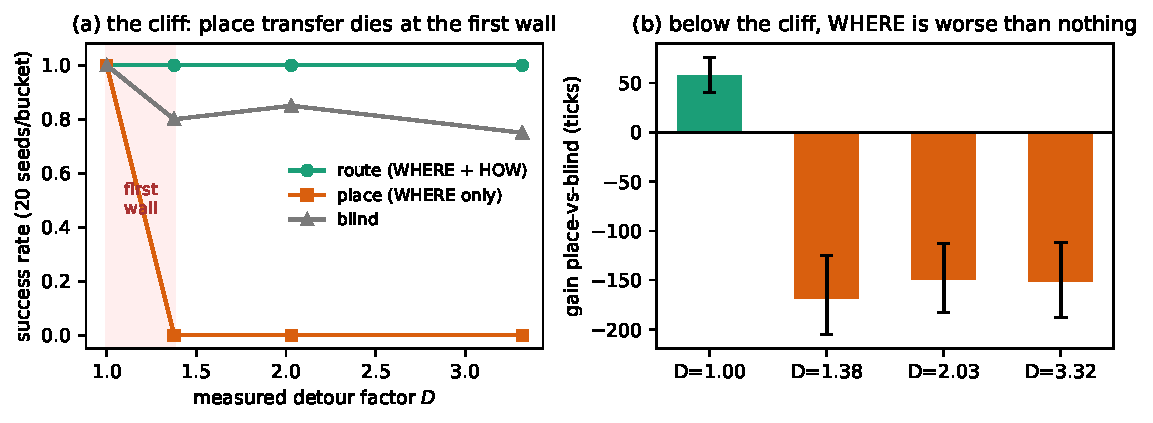
\includegraphics[width=\linewidth]{figures/fig_route_cliff}
\caption{Обрыв (парные плечи на идентичных лабиринтах, 20 сидов на
корзину измеренного обхода). \textbf{(a)} Перенос одних мест не
деградирует с ростом обхода --- он рушится на ПЕРВОЙ же стене,
локализованной пробной корзиной между $D{=}1.00$ и $D{=}1.38$; перенос
маршрута завершает задачу всюду. \textbf{(b)} Ниже обрыва знать ГДЕ
без КАК --- \emph{хуже, чем не знать ничего}: манхэттенская тяга к
известной цели прижимает планировщик к стенам (от $-150$ до $-168$
тиков против слепого исследования), тогда как в открытом мире то же
знание стоит $+57$.}
\label{fig:cliff}
\end{figure}

\begin{table}[h]
\centering
\caption{Три плеча на идентичных лабиринтах (спарены по сиду),
разбитые по ИЗМЕРЕННОМУ фактору обхода $D$; 20 сидов на корзину,
цензурированные выигрыши (отказ $=300$). Перенос одних мест не
деградирует с ростом $D$ --- он рушится на первой стене и там хуже
слепого исследования (манхэттенская тяга к известной цели прижимает
планировщик к стенам). Перенос маршрута завершает задачу всюду; каждое
завершение --- строгий $\rwstar$ с $\phiroute=1$.}
\label{tab:cliff}
\small
\begin{tabular}{lcccc}
\toprule
$D$ & выигрыш маршрут--место [CI] & выигрыш маршрут--слепой [CI] & успех r/p/b \\
\midrule
1.00 & $+4.7$ $[+3.4,+6.0]$ & $+62$ $[+44,+80]$ & 20/\textbf{20}/20 \\
1.38 & $+281$ $[+279,+283]$ & $+113$ $[+77,+155]$ & 20/\textbf{0}/16 \\
2.03 & $+273$ $[+271,+275]$ & $+123$ $[+91,+160]$ & 20/\textbf{0}/17 \\
3.32 & $+262$ $[+259,+264]$ & $+110$ $[+72,+152]$ & 20/\textbf{0}/15 \\
\bottomrule
\end{tabular}
\end{table}

Рисунок~\ref{fig:cliff} показывает обе стороны результата.
Два предзарегистрированных предсказания здесь провалились ---
поучительным образом. Отрицательный контроль при $D{=}1$ был
зарегистрирован в тиках ($|\text{gain}|\le 3$) и дал $+4.7$: зазор ---
это \emph{экономия поворотов} (маршруты BFS идут прямыми отрезками;
планировщик доминирующей оси чередует оси), а не знание маршрута ---
по ДЛИНЕ пути зазор в точности $0.0$ $[0.0,0.0]$ во всех 20 ячейках
открытой сетки. А утверждение <<выигрыш растёт с $D$>> неизмеримо: при
нулевом успехе переноса мест выигрыш насыщается на потолке
цензурирования. Правильная форма закона --- ступенька, локализованная
пробной корзиной в $D\in(1.00,1.38)$, то есть на первой стене.
% re-registration documented in the artifact.

\section{Закон разрыва: где рвётся песня}
\label{sec:rupture}

Свидетель штампует ребро $i$ на тике $i$: его след стареет
неравномерно --- начало маршрута всегда старше конца, --- и путник,
запоздавший на $a_0$, \emph{гонится за угасающей песней}. Под
стандартным гейтом связывающим является ТЕКУЩЕЕ ребро (старейшее из
оставшихся), что даёт три режима по оси $a_0$: завершение; разрыв на
предсказуемом индексе пути; мёртв по прибытии. Предиктор полностью
детерминирован: калибровочный прогон без затухания записывает
кинематику путника (индекс пути на каждый тик, с учётом поворотов), а
зарегистрированное предсказание проигрывает гейт в замкнутой форме по
этой траектории --- тот же приём, который дал $6/6$ на отложенной
выборке сопутствующей статьи.

По 5 лабиринтам $\times$ 11 задержкам $\times$ 2 уровням доверия (110
ячеек, зарегистрированы до исполнения): \textbf{110/110 совпадений
режимов; все 21 разрыв в середине маршрута --- ровно на предсказанном
индексе ребра (ошибка $0$)}; и переброс доверия для маршрутов --- при
доверии $0.7$ масса ребра с однократным проходом даёт
$\mathrm{age}_{\max} = 9.6 < L$, так что \emph{ни один маршрут не
фиксируется вовсе} ($0$ наблюдённых фиксаций; дискретный выключатель
сопутствующего закона, теперь для путей). Разрыв перенесённого
маршрута --- не шум, а закон: те же константы
$(\alpha,\tau,\text{trust})$, которые задают, КОГДА закрывается гейт
варпа мест, задают и то, ГДЕ рвётся маршрутный варп.

\section{Стратификация по опасностям: песня защищает}
\label{sec:hazard}

\begin{table}[h]
\centering
\caption{Открытые поля, густо усеянные проходимыми, но штрафуемыми
опасностями (плотность $0.20$); маршрут свидетеля избегает опасностей
по опыту; 20 парных миров, затухание выключено (ось безопасности
изолирована от оси старения). Оба режима переноса ЗАВЕРШАЮТ задачу ---
ось стен (табл.~\ref{tab:cliff}) и ось опасностей независимы;
различается цена.}
\label{tab:hazard}
\small
\begin{tabular}{lccc}
\toprule
Плечо & попадания в опасности [CI] & завершение & среднее $t$ \\
\midrule
маршрут (чужой безопасный путь) & \textbf{0} (все 20 ячеек) & 20/20 & 16.6 \\
место (только ГДЕ) & 3.25 $[2.45, 4.10]$ & 20/20 & 15.9 \\
слепой & 28.7 & --- & --- \\
\bottomrule
\end{tabular}
\end{table}

\begin{figure}[t]
\centering
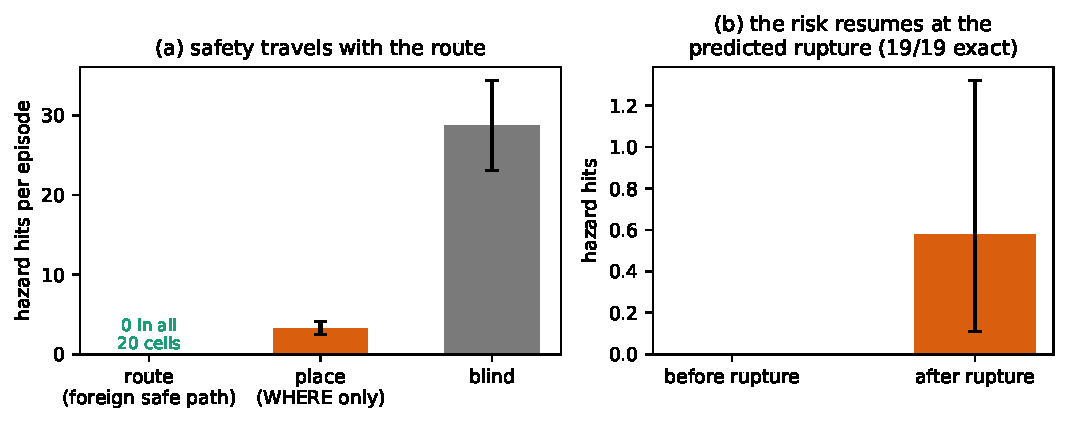
\includegraphics[width=0.92\linewidth]{figures/fig_route_hazard}
\caption{Песня защищает. \textbf{(a)} Попадания в опасности за эпизод:
путник на маршруте свидетеля наследует его безопасность целиком ($0$
во всех 20 мирах); путник с одними местами платит $3.25$ попадания за
то же завершение; слепое исследование платит $28.7$. \textbf{(b)}
Композиция с законом разрыва: в режиме разрыва путник не получает ни
одного попадания, пока длится песня, а после разрыва риск
возобновляется --- и разрыв происходит на предсказанном экспериментом
R2 индексе ребра во всех $19/19$ ячейках.}
\label{fig:hazard}
\end{figure}

Путник, следующий по пути свидетеля, наследует его безопасность
целиком --- за надбавку времени в $+0.7$ тика
(рис.~\ref{fig:hazard}a). Композиция с \S\ref{sec:rupture}: в режиме
разрыва (19/20 миров) путник получает \textbf{0 попаданий до разрыва}
и $0.58$ $[0.11,1.32]$ после него, когда откатывается на знание мест и
заново входит в поле, --- причём все 19 разрывов снова на
предсказанном R2 индексе (ошибка $0$; предиктор с точностью до ребра
воспроизведён на новом классе миров без какой-либо подстройки). Песня
защищает, пока длится, и перестаёт защищать ровно там, где по закону
кончается куплет.

\section{Смысловая идентичность мест}
\label{sec:identity}

Всё сказанное до сих пор --- и всё в сопутствующих статьях ---
держится на общей системе координат. Теперь мы убираем её: приватная
система отсчёта каждого агента --- это истинная сетка под секретным
сдвигом (позже: плюс секретный поворот, кратный $90^\circ$), а
широковещания несут приватные координаты, бессмысленные для
получателя, пока он не решит, что ОЗНАЧАЮТ места отправителя.

\paragraph{Отпечатки и рукопожатие.} Отпечаток места --- это локальная
семантическая констелляция вокруг посещённой клетки: какие
содержательные теги (опасности, стены, вода) стоят на каких
относительных смещениях; он трансляционно-инвариантен и свободен от
координат. Сопоставление \emph{взаимно уникально} (пара принимается,
только если каждая сторона --- единственный кандидат другой стороны
выше порога точного равенства; отправитель знает куда больше мест, чем
получатель, и односторонняя уникальность алиасирует далёкие
<<двойники>> в окрестность получателя), отпечаткам нужно $\ge 2$
значимых ключей, а сдвиг системы отсчёта --- модальная дельта $\ge 3$
согласующихся пар. Ориентиры обязаны нести хотя бы один
СОДЕРЖАТЕЛЬНЫЙ тег: узоры из одной лишь границы (<<пустота>>)
описывают форму мира, а не место, и исключаются --- урок угловой
ловушки ниже.

\paragraph{Результаты свидетель--путник.} По 4 смещениям $\times$ 2
плотностям опасностей $\times$ 10 сидам: семантический выравниватель
восстанавливает секретное смещение \emph{точно в 100\%} прогонов в
мирах с ориентирами (в среднем $15.1$ взаимной пары) и всякий раз
завершает задачу со строгим $\wstar$ ($\varphi{=}1$); координатный
бейзлайн при любом ненулевом смещении в $100\%$ прогонов захватывает
клетку без воды (его редкие <<успехи>>, $6.7\%$, --- это смещённый
маршрут, случайно пересекающий настоящую воду). В алиасированном мире
(безликая внутренняя полоса) два режима идентичности ломаются в
ПРОТИВОПОЛОЖНЫХ направлениях: семантическая идентичность не делает
\emph{ни одного} захвата --- отказывает закрытым образом, --- тогда
как координатная продолжает уверенно захватывать неверные клетки ---
отказывает открытым. Именно эта асимметрия, а не сырая точность, ---
самый глубокий аргумент в пользу смысловой идентичности: когда мир не
поддерживает опознание, семантическая система это знает.

\subsection{Полный стек и снятие последней оси}
\label{sec:stack}

\paragraph{Онлайн-выравнивание в peer-стеке.} При $N{=}4$ агентах в
условиях дефицита, каждый в своей секретной системе отсчёта,
выравнивание складывается ПО ХОДУ эпизода: агенты исследуют, совместно
посещённые ориентиры накапливаются, и системы отсчёта по каждому
отправителю защёлкиваются посреди прогона (наступление в $100\%$
эпизодов, средний тик ${\approx}15$). Объединённый успех: оракул с
общей системой отсчёта $0.456$, координаты при рассогласовании
$0.350$, семантика $0.444$ --- \textbf{возвращено 88\% зазора}, со
строгим $\wstar$, работающим через восстановленные системы отсчёта.

\paragraph{Закон без системы отсчёта.} Перезапуск сопутствующего
закона расстояния с гейтом доверие$\times$давность ПОВЕРХ
семантической идентичности при смещении системы отсчёта даёт точки
излома $20/14/9$ --- \emph{в точности те же целые числа, что и
замкнутая форма при общей системе отсчёта}. Гейт и восстановление
системы отсчёта --- ортогональные слои: закон не замечает, что общая
сетка исчезла.

\paragraph{$SE(2)$: без общего севера.} С добавлением секретных
поворотов одна гипотеза поворота на каждые $90^\circ$ переиспользует
трансляционный выравниватель, а победитель обязан \emph{доминировать}
($\ge 2\times$ консенсуса ближайшего конкурента). Результаты: точное
восстановление $(r^\ast,\delta^\ast)$ в \textbf{80/80} комбинациях
поворот$\times$смещение$\times$сид со $100\%$ завершением со строгим
$\wstar$; в $180^\circ$-симметричном мире --- где система отсчёта
невосстановима \emph{в принципе} --- выравниватель отказывается
($0/10$ захватов), тогда как координаты отказывают открытым образом
($10/10$ неверных захватов); и закон расстояния снова ничего не
замечает ($\mathrm{bp}=20$ при свидетеле, повернутом на $90^\circ$).
Чисто трансляционный выравниватель, для контраста, никогда не
восстанавливает повернутую систему отсчёта ($0/60$), но не всегда
отказывает закрытым образом: в $2/60$ ячеек $180^\circ$-симметричная
подструктура опасностей позволяет ему отказать ОТКРЫТЫМ ---
эмпирическая мотивация правила доминирования.

\begin{figure}[t]
\centering
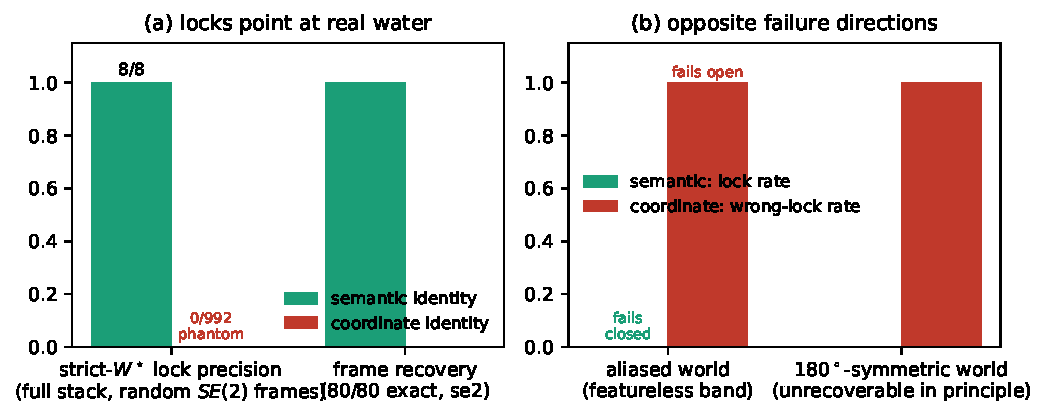
\includegraphics[width=0.92\linewidth]{figures/fig_route_identity}
\caption{Смысловая идентичность при $SE(2)$-системах отсчёта.
\textbf{(a)} Каждый строгий $\wstar$-захват семантического стека
указывает на настоящую воду ($8/8$); координатный стек делает $992$
захвата, и все --- фантомы ($0/992$); само восстановление системы
отсчёта точно в $80/80$ комбинаций свидетель--путник. \textbf{(b)}
Асимметрия отказов в мирах, где опознание невозможно (безликая полоса;
$180^\circ$-симметричная планировка, где система отсчёта
невосстановима в принципе): семантическая идентичность отказывается
захватывать --- отказывает закрытым образом, --- тогда как
координатная продолжает уверенно захватывать неверные клетки ---
отказывает открытым.}
\label{fig:identity}
\end{figure}

\paragraph{Угловая ловушка.} В полном стеке сырой успех
недискриминативен при поворотах (повернутый координатный <<яд>>
большей частью отображается за пределы сетки и вырождается в
псевдоисследование), поэтому зарегистрированный дискриминатор ---
\emph{точность варп-захватов}: доля строгих $\wstar$-захватов,
указывающих на настоящую воду. До фильтра пустоты ранние граничные
отпечатки (агенты стартуют в углах; границы прямоугольника
$180^\circ$-симметричны) питали гипотезы неверной системы отсчёта, и
семантическая точность была $0.159$; с исключением границ как
не-ориентиров она равна \textbf{$1.000$ ($8/8$) против $0.000$
($0/992$ фантомных захватов) у координат}, с наступлением
выравнивания в $100\%$ эпизодов и чистыми регрессиями на всех более
ранних экспериментах (рис.~\ref{fig:identity}).

\section{Связанные работы}
\label{sec:related}

\paragraph{Слияние карт и распознавание мест.} Мультироботный SLAM
трактует межкартовую ассоциацию данных как задачу оценивания над
метрическими признаками~\cite{cadena2016slam}; визуальное
распознавание мест~\cite{lowry2016vpr} сопоставляет внешний вид. Наш
вклад --- не конкурирующий сопоставитель, а измерительный слой поверх:
завершение, обусловленное провенансом, через восстановленные системы
отсчёта; асимметрия <<отказ закрытым/открытым образом>> как
зарегистрированное предсказание; инвариантность закона при удалении
системы отсчёта.
\paragraph{Обмен маршрутами.} Стигмергия переносит пути анонимно
(градиенты феромонов); обучаемая коммуникация (например,
CommNet~\cite{sukhbaatar2016commnet}) переносит политики непрозрачно.
Ни та, ни другая не выставляет разложение по провенансу рёбер, поэтому
ни та, ни другая не может сказать --- тем более предсказать, --- где
рвётся перенесённый маршрут. Предиктор разрыва --- это идея Time
Warp~\cite{jefferson1985}, применённая к затуханию памяти:
детерминированное проигрывание гейта по калиброванной кинематике.
\paragraph{Сонглайны.} Нарративная рамка теперь несущая в обоих
направлениях: песня --- это последовательность (маршрутный варп), её
места опознаются по смыслу (семантическая идентичность), она угасает
куплет за куплетом (закон разрыва) и защищает идущего, пока длится
(стратификация по опасностям).
% TODO: add refs: ProcTHOR/ALFWorld for future substrates.

\section{Ограничения и честные отрицательные результаты}
\label{sec:limits}

(1) Сеточные миры; только сдвиги и повороты на $90^\circ$ ---
непрерывное $SE(2)$ и шум внешнего вида остаются будущей работой
(порог отпечатков --- точное равенство, поскольку субстрат бесшумен;
шумным субстратам нужна машинерия зазоров из области распознавания
мест). (2) Четыре зарегистрированных предсказания провалились и
сообщаются вместе с механизмами: отрицательный контроль $D{=}1$ в
тиках (экономия поворотов; точен по длине пути), монотонность выигрыша
по $D$ (цензурирование; истина --- обрыв), сравнение успеха полного
стека при поворотах (недискриминативно; заменено точностью захватов) и
<<трансляция отказывает закрытым образом>> ($2/60$ отказывают открытым
через симметричные подструктуры). (3) Следование по маршруту --- новый
ярус планировщика; все три плеча делят его, но ценность маршрутного
варпа измерена относительно именно этого потребителя. (4) Безопасность
по опасностям переносится по построению, когда маршрут свидетеля
безопасен; измеренное содержание --- в том, что перенос мест НЕ МОЖЕТ
её нести и что защита кончается на предсказанном разрыве. (5)
Завершение варп-захватов на уровне дефицита по-прежнему управляется
феноменологией столкновений из сопутствующей статьи.

\section{Заключение}

Сведите песню к точке на общей карте --- и незаметно ломаются две
вещи: КАК (фатально на первой же стене, дорого в любом поле
опасностей) и КТО-ЧТО-ИМЕЕТ-В-ВИДУ (фатально при любом рассогласовании
систем отсчёта --- и опасно именно потому, что отказывает открытым
образом). Верните песню --- рёбра с провенансом, места со смыслом ---
и оба отказа становятся измеримыми, закономерными и в значительной
мере исправленными: маршруты переносят завершение и безопасность и
рвутся только там, где велит закон старения; смысл восстанавливает
системы отсчёта точно, честно отказывается, когда мир неоднозначен, и
переносит весь измерительный стек --- $\varphi$, гейты, закон
расстояния --- без изменений в мир, где агенты не делят никаких
координат. Точка никогда не была памятью. Память --- это песня.

\appendix

\section{Зарегистрированные предсказания и ревизии}
\label{app:registered}
Все предсказания были записаны на диск до исполнения; артефакт
сохраняет обе версии всюду, где операционализация пересматривалась.
Ревизии: отрицательный контроль R1 перемерен по длине пути;
монотонность выигрыша R1 переформулирована как детекция обрыва;
дискриминатор полного стека W9 сменён с успеха на точность
варп-захватов; функционирование строгого $\wstar$ в W8 расширено на
варп-ассистированные собственные завершения (такси-цепочки).
% TODO: inline the registration JSONs.

\section{Воспроизводимость}
\label{app:repro}
\begin{verbatim}
PYTHONPATH=. python experiments/warp/exp_route_warp_r0.py
PYTHONPATH=. python experiments/warp/exp_route_warp_r1.py --seeds 20
PYTHONPATH=. python experiments/warp/exp_route_warp_r2.py --seeds 5
PYTHONPATH=. python experiments/warp/exp_route_warp_r3.py --seeds 20
PYTHONPATH=. python experiments/warp/exp_warp_semantic_identity.py
PYTHONPATH=. python experiments/warp/exp_warp_semantic_stack.py --seeds 20
PYTHONPATH=. python experiments/warp/exp_warp_rotation.py --seeds 10
\end{verbatim}

\begin{thebibliography}{9}

\bibitem[Cadena et~al.(2016)]{cadena2016slam}
C.~Cadena, L.~Carlone, H.~Carrillo, Y.~Latif, D.~Scaramuzza,
J.~Neira, I.~Reid, and J.~J. Leonard.
\newblock Past, present, and future of simultaneous localization and
mapping: Toward the robust-perception age.
\newblock \emph{IEEE Transactions on Robotics}, 32(6):1309--1332, 2016.

\bibitem[Jefferson(1985)]{jefferson1985}
D.~R. Jefferson.
\newblock Virtual time.
\newblock \emph{ACM Transactions on Programming Languages and Systems},
7(3):404--425, 1985.

\bibitem[Lowry et~al.(2016)]{lowry2016vpr}
S.~Lowry, N.~S\"underhauf, P.~Newman, J.~J. Leonard, D.~Cox,
P.~Corke, and M.~J. Milford.
\newblock Visual place recognition: A survey.
\newblock \emph{IEEE Transactions on Robotics}, 32(1):1--19, 2016.

\bibitem[Sukhbaatar et~al.(2016)]{sukhbaatar2016commnet}
S.~Sukhbaatar, A.~Szlam, and R.~Fergus.
\newblock Learning multiagent communication with backpropagation.
\newblock In \emph{NeurIPS}, 2016.

\end{thebibliography}

\end{document}
